% Find the bundled IEEE class alongside the other supporting assets.
\makeatletter
\def\input@path{{artifacts/}}
\makeatother
\documentclass[conference]{IEEEtran}
\usepackage{cite}
\usepackage{amsmath,amssymb}
\usepackage{graphicx,booktabs,array}
\usepackage{newtxtext,newtxmath}
\usepackage[hidelinks]{hyperref}
\usepackage[section]{placeins}
\usepackage{tikz}
\usetikzlibrary{arrows.meta,positioning}
\graphicspath{{artifacts/}}
\title{Improving Dynamic Memory Allocation in PIM-malloc}
\author{
\IEEEauthorblockN{\small
Bhavya Negi (\textit{230101025}), Lasya Madhu Sundar (\textit{230101058}),
Pinjala Narmada (\textit{230101074}), Tedla Mahaswin (\textit{230101104})}
\IEEEauthorblockA{\small \textit{Group-11}}
}
\begin{document}
\raggedbottom
\maketitle

\begin{abstract}
PIM-malloc provides dynamic memory allocation for processing-in-memory systems, where each processor has a small scratchpad and its own local DRAM. We study changes to its software allocator. These changes cover empty-page retention, page lookup, a new slab class for medium-sized objects, and placement of buddy metadata in the scratchpad. We first reproduce the paper's allocation benchmark, then use a common corrected implementation to compare the changes. The evaluation includes allocation microbenchmarks, graph kernels, Larson workloads and a cache trace. We report execution time, memory traffic and memory use, and examine where each change helps and where its overhead becomes a problem.
\end{abstract}
\begin{IEEEkeywords}
processing-in-memory, dynamic memory allocation, buddy allocator, slab allocation
\end{IEEEkeywords}

\section{Introduction}
Moving data between a CPU and DRAM can cost more time and energy than the computation itself. Processing-in-memory (PIM) places processors close to memory so that they can work on local data. This is useful for workloads such as graph updates, where the program accesses many small pieces of data.

These programs also need dynamic memory allocation. A graph may need more space when edges arrive, while a cache must allocate and free objects as its contents change. On a PIM device, the allocator must manage local memory using a much smaller processor and scratchpad than a CPU has available.

Our baseline is \emph{PIM-malloc: A Fast and Scalable Dynamic Memory Allocator for Processing-In-Memory (PIM) Architectures} by Lee et al.~\cite{pimmalloc}. The paper studies where allocation should run and where its metadata should stay. Its software design uses a local frontend for small objects and a shared buddy backend for larger blocks. The paper also proposes a hardware metadata cache. Our project changes the software design and uses the released simulator~\cite{artifact}.

We focus on four questions. Can we avoid scanning pages during allocation and free? How much empty memory should each tasklet retain? Can a slab serve requests that currently go straight to the backend? Can a small amount of WRAM reduce the backend's metadata traffic? We implement these changes separately and together. The report first explains the baseline, then describes our design and experiment setup. Section~\ref{sec:evaluation} contains the performance results and their analysis.

\section{Background}
\subsection{DPUs and their memory}
In the UPMEM system studied by the paper, a \emph{DPU}, or DRAM Processing Unit, is a small processor attached to a local DRAM bank. It runs at 350 MHz and supports up to 24 hardware threads, called \emph{tasklets}. Tasklets on one DPU share its memory. A tasklet cannot directly access another DPU's memory~\cite{pimmalloc}.

A DPU has three main memory regions. MRAM is the large local DRAM bank that holds application data. WRAM is a fast 64 KiB scratchpad used for working data, stacks and software state. IRAM is the 24 KiB instruction memory. Programs move data between MRAM and WRAM using explicit DMA transfers. Normal load and store instructions operate on WRAM. This makes metadata placement important: repeatedly reading a small item from MRAM can be expensive even when the item itself occupies little space.

Each DPU manages its own address space. A system with many DPUs therefore needs many separate heaps. Our experiments study the allocator within one DPU, where several tasklets share a heap in MRAM.

\subsection{Dynamic allocation and the buddy algorithm}
An allocator returns a block when a program requests memory and makes that block available again after free. It also maintains \emph{metadata}: block sizes, free/used state, ownership information and links between pages. This metadata is separate from the application's payload.

A buddy allocator divides a heap into power-of-two blocks. To satisfy a small request, it splits a larger free block until it reaches the required size. On free, it merges adjacent buddy blocks when both are free. A tree records these states. This supports different request sizes and allows the allocator to recover large contiguous blocks.

However, an allocation or free may visit several tree levels. If the tree stays in MRAM, those visits require transfers. Sharing the backend also requires synchronization between tasklets. PIM-malloc places a frontend above this backend to reduce how often applications pay these costs.

\subsection{The PIM-malloc frontend and backend}
The released software frontend has eight power-of-two size classes, from 16 B to 2 KiB. Each tasklet has its own frontend state. A class obtains a 4 KiB page from the backend and divides it into object slots. Each page has a 24 B header and a 128-bit allocation bitmap. The frontend can then satisfy several requests from the same page.

The backend manages the shared MRAM heap using the buddy algorithm. A mutex protects its tree. The released design packs two bits per tree node and uses a 64 B WRAM buffer to read and update metadata from MRAM. Requests above 2 KiB bypass the small-object frontend and call buddy directly. Figure~\ref{fig:baseline-path} shows these paths.

\begin{figure}[t]
\centering
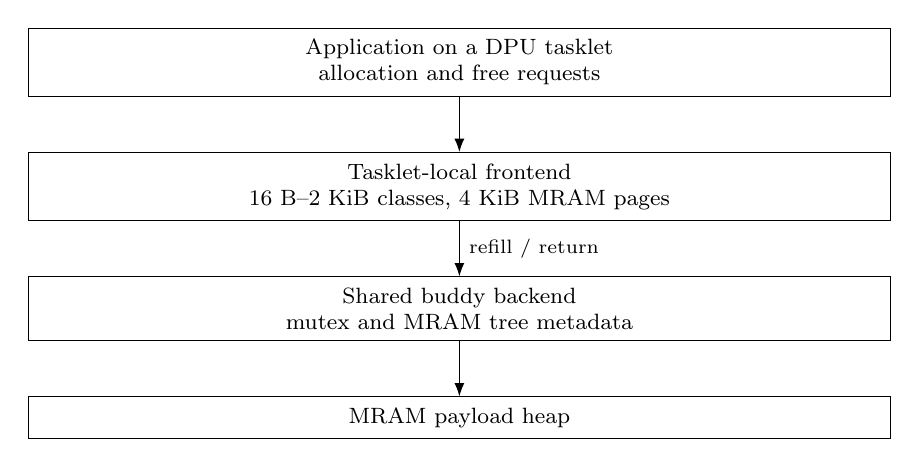
\begin{tikzpicture}[node distance=7mm, every node/.style={font=\footnotesize}, box/.style={draw,align=center,text width=.88\columnwidth,inner sep=4pt}, >={Latex}]
\node[box] (app) {Application on a DPU tasklet\\allocation and free requests};
\node[box,below=of app] (front) {Tasklet-local frontend\\16 B--2 KiB classes, 4 KiB MRAM pages};
\node[box,below=of front] (back) {Shared buddy backend\\mutex and MRAM tree metadata};
\node[box,below=of back] (heap) {MRAM payload heap};
\draw[->] (app)--(front);
\draw[->] (front)--node[right]{\scriptsize refill / return}(back);
\draw[->] (back)--(heap);
\end{tikzpicture}
\caption{Baseline allocation path; requests above 2 KiB go directly to the backend. DPU = DRAM Processing Unit; MRAM = main DRAM; DRAM = dynamic random-access memory; B = bytes; KiB = 1024 bytes.}
\label{fig:baseline-path}
\end{figure}

This leaves several possible costs. A frontend may scan many pages to find a free slot or to identify a pointer during free. Returning an empty page immediately can cause another backend call soon afterward. Keeping every empty page can waste heap space. Finally, requests beyond the frontend's size limit still use buddy for every object. Our changes target these parts of the allocator.

\section{Proposed Design}
\subsection{Common implementation and memory limits}
Free and reuse must work consistently across variants; otherwise timings can confuse a policy change with incorrect reclamation.

We corrected bitmap indexing, free routing and empty-page unlinking in the common implementation. We also added correct handling of large backend blocks and nonfatal allocation failure. Every contribution variant uses these same fixes.

The released simulator allows 256 KiB WRAM and reserves 24 stacks of 4 KiB. We retain that setup for the original-paper reproduction. For our changes, we cap WRAM at 65,536 B and use 1,536 B reservations for each of the 24 stacks. The original reproduction and the contribution experiments are therefore separate baseline families. This address limit checks the linked memory budget. Worst-case stack use and physical instruction-memory fit still need hardware validation.

\subsection{Empty-page retention}
Empty pages trade reuse against capacity. Returning them immediately can force the next burst back to the shared backend. Keeping them avoids refills but holds memory within one tasklet and class. Bounded retention aims to keep useful pages while releasing idle capacity.

We implemented eager population, immediate return, fixed retention and adaptive retention. Fixed-2 keeps at most two completely empty pages per class. It does not limit the number of live or partially filled pages. When a page fills, the frontend can obtain another page and use all its slots.

Demand can move between classes, so a fixed limit may retain pages where they are no longer useful. The adaptive policy maintains a target for each class. Repeated refills increase that target. Periodic checks lower idle targets and return excess empty pages. A shared byte budget limits total retained memory per tasklet. A pressure flag at 75\% heap use and an emergency drain allow further reclamation. A tasklet only reclaims its own pages. This keeps ownership simple but can leave memory with an inactive tasklet.

Periodic checks keep maintenance off most requests, at the cost of slower reclamation. We support checks every 64 or 128 allocator operations. An operation means one allocation or one free. Changing the interval changes both maintenance overhead and how quickly an idle target decays.

\subsection{Indexed page lists and ownership lookup}
A larger page pool can make discovery more expensive. Allocation needs a page with free space, while free needs the owner of a known pointer. Separate lists and a pointer-derived table answer these questions directly instead of repeating a scan.

We replace page scans with separate partial, full and empty lists. Allocation can start from a partial or empty page. Filling or emptying a page moves it between lists by updating a few links. We also add an ownership table indexed by the pointer's 4 KiB heap leaf. An 8 B entry identifies the tasklet, class and page or span head, so free can find the right frontend directly.

A 32 MiB payload heap has 8,192 leaves, giving a 64 KiB ownership table in MRAM. This is extra metadata outside the payload heap. The lists add 24 B of WRAM state per tasklet and class. Frees remain local to the tasklet that allocated the object.

\subsection{A slab class for 4 KiB objects}
Requests above 2 KiB bypass the original frontend and pay for buddy traversal and locking per object. A larger span can pay that cost once for several slots. We add a separate class to target these requests while preserving small-object layouts, and compare span sizes to examine the space cost.

The original frontend ends at 2 KiB. We add a ninth class for requests from 2,049 B through 4,096 B. It obtains a 16, 32 or 64 KiB MRAM span and divides that span into 4 KiB slots. For span size $S$ and slot size $B$, the existing header and bitmap give
\begin{equation}
 C(S,B)=\min\left(128,\left\lfloor\frac{S-24}{B}\right\rfloor\right).
\end{equation}
The three span sizes hold 3, 7 and 15 objects. Smaller classes keep their original 4 KiB pages, and requests above 4 KiB still call buddy directly.

The span records its size, and the ownership table maps every covered leaf to its head. Retention charges the span's physical bytes: an empty 64 KiB span costs sixteen 4 KiB units. All variants receive the same byte budget within a comparison. Geometry stays fixed during a run, and live objects do not move. We first tested slabs separately, then added them to the indexed allocator with both retention policies.

\subsection{Buddy metadata in WRAM}
Backend calls remain after slab reuse. Many paths share upper buddy-tree levels, making their metadata a useful reuse target. Pinning the whole tree would compete with application data and stacks in WRAM. We therefore keep only a small upper prefix, leaving lower metadata in MRAM.

We keep tree levels 0--10 in shared WRAM and continue to stream lower metadata from MRAM. For the 32 MiB heap, the upper levels need 524 B, rounded to a 528 B DMA boundary. The aligned prefix includes the first packed word of the next level. Two descriptor fields add 8 B. Alignment accounts for a further 4 B in the measured memory layout.

The WRAM copy holds the current upper-tree state. Lower DMA windows cannot overlap it. The existing buddy mutex protects updates. An explicit checkpoint copies the prefix to its MRAM shadow when the allocator is locked or idle. Normal allocations do not write the prefix back after every access.

This is a software placement change that uses additional WRAM. The baseline paper's hardware cache uses dedicated cache and instruction support. We do not implement that hardware mechanism. We also leave backend sharding, lifetime regions, cross-DPU balancing and online class resizing for future work. A small bitmap-cache layout probe was considered but was not part of the measured allocator.

\section{Experimental Methodology}
\subsection{Setup and comparison stages}
We use the released software simulator at 350 MHz with one DPU and SDK 2023.2.0. The original Figure 15 reproduction uses the authors' allocator bodies and memory layout. Contribution experiments share the corrected paths and the 64 KiB WRAM limit described above.

The final matrix has 14 workload settings and seven variants per setting, for 98 configurations. Each comparison uses the same input and 32 MiB payload heap. Final adaptive variants check every 64 allocation-plus-free operations. All final variants have a 256 KiB empty-byte budget per tasklet and a maximum of two empty pages or spans per class. Earlier retention/indexing studies used 16 KiB per tasklet. The paired interval study compares 64 with 128 operations. The combined slab-size and heavy-request studies use interval 128 and 256 KiB. We compare times only within a stage.
The plot labels use B for scan fixed-2, I for indexing, S for indexing plus slabs, and P for indexing plus slabs and pinned metadata. The suffix A means adaptive-64; F means fixed-2.

\subsection{Workloads}
The allocation microbenchmark follows the paper: 128 requests per tasklet, sizes of 32 B, 256 B and 4 KiB, and one or sixteen tasklets. The two graph insertion kernels also follow the paper's data structures. We reservoir-sample 3,072 real undirected Gowalla edges, preload 2,048, and insert 1,024 while storing both directed arcs. Linked blocks request 256 B. Growing arrays start at 64 B and reach 256 B in this small sample. The full paper uses larger graphs and arrays.

Larson follows the persistent-pool replacement pattern~\cite{larson,mimalloc}. The original port uses 8--999 B requests. Two explicit configurations use 8--4095 B and 8--8191 B, with 64 objects per tasklet, four pool-length warmups and 256 timed replacements per tasklet. The larger ranges are benchmark settings, not changes to a saved trace.

The CloudPhysics cache uses original variable I/O lengths and request order from a public sample~\cite{cloud}. It processes full payloads but omits storage and arrival timing. Graph churn uses deletion and reinsertion inspired by faimGraph~\cite{faim}. PrIM selection~\cite{prim} processes 32,768 items in four passes with preallocated output, providing a control with no work-phase allocation.

The KV-growth case replays allocation of 512 B blocks for 128 prompt and 256 output tokens, with one block per token per tasklet as an explicit assumption. The released artifact does not supply the complete attention kernel or serving trace. This replay excludes attention computation and serving latency. Dense bursts, persistent pools, changing class demand and sparse survivors provide additional allocator tests.

\subsection{Measurements and checks}
Zero-instruction labels mark allocation, free and program phases. \emph{Work time} is the concurrent application-phase makespan. \emph{Total time} also includes initialization, preload or warmup, output checking and final free/drain. A speedup divides the baseline time by the variant time for the same phase. Mean individual allocation latency is a separate metric because tasklet requests overlap.

DRAM counters cover the full execution, including final accounting. They count memory commands, often 8 B each, rather than source-level DMA calls. They exclude WRAM accesses, instruction fetch and host transfers. Payload peaks also exclude the ownership table and buddy metadata, which we report separately.

Native sanitizer and differential tests check live intervals, payloads, wrong-size frees, graph membership and backend tree state. DPU runs check offered work, final ownership/list state, zero live payload and full buddy coalescing. Expensive invariant walks stay outside performance work. We check source, simulator and trace hashes. Fixed-input simulations are deterministic, so repeated runs do not provide independent confidence intervals. Extra seeds and trace windows test input sensitivity.

\section{Evaluation}\label{sec:evaluation}
\subsection{Reproducing the paper baseline}
Table~\ref{tab:baseline} compares the original Figure 15 labels with our measurements. Across the buddy and software allocator settings, the maximum absolute deviation is 7.20\%. The table shows the software allocator; the accompanying baseline results contain both allocators. The displayed latency is batch completion time divided by 128 requests per tasklet. The paper does not state the exact multithread aggregation formula, so this is our documented interpretation. Individual request latencies remain available separately. These numbers use the preserved runtime and are separate from our contribution baseline.
\begin{table}[t]
\caption{Software allocator reproduction. Latency is batch time / 128, in microseconds. B = bytes; KiB = 1024 bytes. Tasklets are hardware threads.}\label{tab:baseline}
\centering\small
\begin{tabular}{rlrr}\toprule
Tasklets & Request & Paper & Reproduced \\ \midrule
1 & 32 B & 6.9 & 6.99 \\
1 & 256 B & 32 & 32.12 \\
1 & 4 KiB & 310 & 312.71 \\
16 & 32 B & 51 & 51.86 \\
16 & 256 B & 430 & 457.72 \\
16 & 4 KiB & 6700 & 6808.97 \\
\bottomrule\end{tabular}
\end{table}

The key size boundary is 2 KiB: smaller requests use the software frontend, while 4 KiB requests still use buddy directly. Our later slab change targets this missing frontend class. The original reproduction establishes the starting behavior; the corrected scan fixed-2 control is the baseline for our final contributions.

\subsection{Retention, indexing and check frequency}
On regular four-tasklet phases, fixed-2 takes 16.25 ms total and adaptive takes 18.52 ms. Both peak at 128 KiB. Eager population takes 29.66 ms at 192 KiB, while immediate return takes 23.82 ms at 96 KiB. Fixed retention works well when demand is stable and pages are reused predictably.

Adaptation is more useful when demand changes. In the four-tasklet class-handoff test, indexed adaptive takes 101.04 ms with 344 refills, compared with 113.76 ms and 400 refills for indexed fixed-2. In a tight-heap test, adaptive completes at one tasklet while fixed-2 misses twelve requests. At four tasklets, adaptive still misses eight requests, compared with forty-eight for fixed-2. We compare those cases by completed work, since their runtimes alone would be misleading.

Figure~\ref{fig:index} isolates lists and ownership lookup with fixed retention. For Larson at one tasklet, work falls from 202.945 ms with scans to 69.812 ms with lists, 166.219 ms with lookup alone, and 38.759 ms with both, a 5.24-fold speedup. Graph churn falls from 2055.865 to 236.009 ms with lists, 1902.033 ms with lookup alone, and 89.790 ms with both. The combined gain is \textbf{22.90-fold}. Lists avoid allocation scans and lookup reduces free-side search. The two changes therefore work well together. This one-tasklet ablation uses the earlier input and budget; it is separate from the final four-tasklet churn comparison.

On a stable resident pool, indexed fixed takes 69.72 ms and indexed adaptive takes 74.50 ms. Indexing removes search overhead in both policies, but it does not remove adaptive maintenance. This explains why fixed-2 can remain faster even after both use the same page lookup.
\begin{figure}[t]
\centering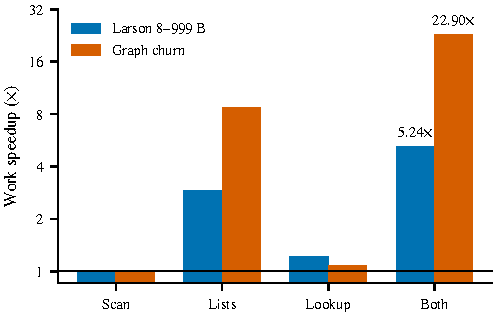
\includegraphics[width=\columnwidth]{index-ablation.pdf}
\caption{Indexing ablation at one tasklet with fixed-2 retention, relative to the scan control. B = bytes; Both = page lists plus ownership lookup.}
\label{fig:index}
\end{figure}

Increasing the check interval from 64 to 128 operations gives only small improvements. Most main-seed cases improve by 0.30--0.83\%, while four-tasklet linked insertion becomes 1.30\% slower. One-tasklet Larson changes from 42.161 to 41.811 ms, still behind indexed fixed-2 at 38.759 ms. Its DRAM commands change from 200,230 to 200,234, so lower traffic does not explain the time saving. Fewer maintenance instructions and changed scheduling are plausible causes. The longer interval also slows idle decay. The final matrix returns to interval 64.

In the second-seed checks, Larson and churn improve by 0.44--0.60\%. PrIM selection is nearly unchanged because it makes no work-phase allocator calls. Most pairs have unchanged refill counts and DRAM bytes. Thus, reducing check frequency is a small tuning change, while removing page scans addresses a much larger cost.

\subsection{Slab size, request sizes and capacity}
The standalone slab tests first confirmed that combining several 4 KiB objects into one backend allocation reduces repeated buddy calls. In the combined four-tasklet dense burst, fixed retention takes 136.669 ms with direct allocation, 35.950 ms with 16 KiB spans, 11.947 ms with 32 KiB spans, and 4.633 ms with 64 KiB spans. All use the same 256 KiB empty-byte budget. The memory cost is substantial: two surviving 4 KiB objects can keep 128 KiB reserved in separate large spans.

A 64 KiB heap holds sixteen direct 4 KiB objects, but only twelve, fourteen or fifteen objects with the three slab layouts because of headers and unused tails. A fragmented heap may also lack a sufficiently large contiguous span. The implementation has no hidden direct-allocation fallback.

\subsection{Repeated allocation and persistent pools}

\begin{figure}[t]
\centering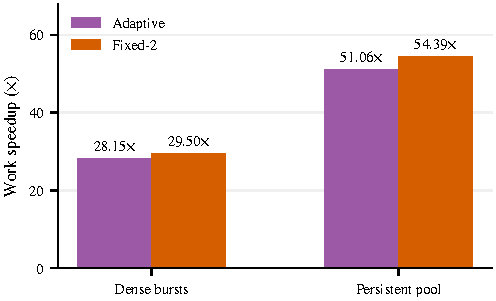
\includegraphics[width=\columnwidth]{reuse-summary.pdf}
\caption{Synthetic reuse at four tasklets. Each 64 KiB slab variant uses its matching indexed direct control, interval 128 and equal byte budget. KiB = 1024 bytes; fixed-2 retains at most two empty spans per class.}
\label{fig:synthetic}
\end{figure}

\begin{figure*}[!t]
\centering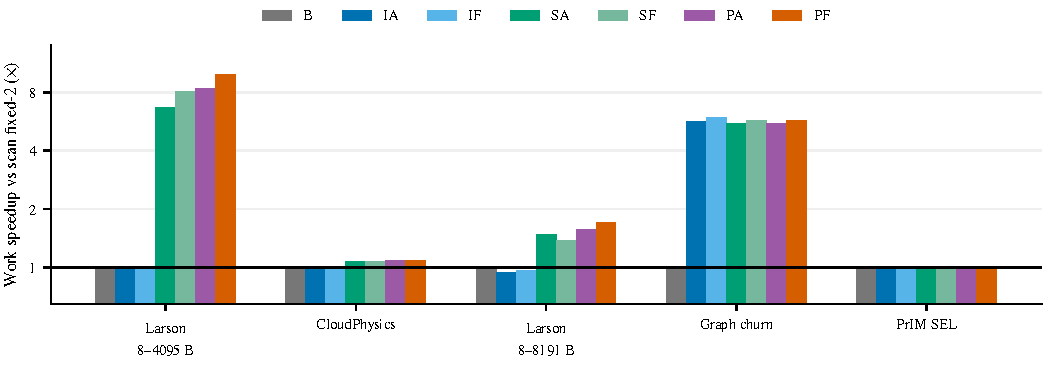
\includegraphics[width=\textwidth]{final-progression.pdf}
\caption{Final work speedups at four tasklets, relative to B. B = scan fixed-2; IA/IF = indexed adaptive-64/fixed-2; SA/SF add slabs; PA/PF also add pinning. PrIM = Processing-in-Memory benchmarks; SEL = selection; B in request sizes = bytes.}
\label{fig:progression}
\end{figure*}

Figure~\ref{fig:synthetic} shows the larger gains in the combined synthetic tests. At four tasklets, 64 KiB slabs improve dense-burst work by \textbf{29.50-fold} with fixed retention and 28.15-fold with adaptive retention. The corresponding total gains are 23.95-fold and 23.00-fold. Backend allocations fall from 512 to 24. Each tasklet allocates and frees 32 objects over four rounds, allowing empty spans to be reused.

The persistent pool has 64 live 4 KiB objects per tasklet and 128 random victim replacements per tasklet. With fixed retention, slab reuse improves work from 137.603 to 2.530 ms, or \textbf{54.39-fold}; adaptive improves it by 51.06-fold. Total gains are 26.94-fold and 26.23-fold. Here, direct allocation calls buddy for every replacement, while a freed slot can be reused within its slab. The live payload stays at 1,024 KiB, but the slab pool reserves 1,280 KiB at the work-end snapshot.

These tests show when the slab mechanism is most useful: many requests in the new class, repeated reuse and enough live objects to fill spans. They do not represent complete application speedups. The sparse case also becomes faster, but its two survivors keep sixteen times their live payload reserved. Larger slabs trade backend work for reserved memory rather than removing both costs.

\subsection{Transferring slabs to mixed-size workloads}

The unchanged small-request ports do not use the new class. Larson 8--999 B becomes about 4.7--5.5\% slower and churn 3.1--4.2\% slower, with unchanged refills and bytes. The reduced graphs request at most 256 B, and selection allocates nothing during work. Adding a class for larger objects cannot help these request patterns.

The explicit Larson 8--4095 B configuration has 523 slab-eligible allocations out of 1,024 timed allocations at four tasklets. With interval 128, 64 KiB fixed slabs reduce work from 159.826 to 19.894 ms, an 8.03-fold gain over the matching indexed control. A 32 KiB slab takes 20.221 ms, so increasing an already useful slab is a much smaller part of the gain. Some adaptive cases prefer 32 KiB. CloudPhysics has only 54 eligible requests out of 150, with 43 above 4 KiB. Its fixed work changes from 122.784 to 114.528 ms, a 1.07-fold gain. Payload processing and bypass requests leave less time for slabs to save.

\subsection{The full allocator}

Figure~\ref{fig:progression} compares all seven requested stages at four tasklets. The full fixed variant reaches 9.849-fold work speedup on Larson 8--4095 B. Indexing alone is almost neutral there because many requests bypass the original small classes. The new slab class provides most of the gain. Wider Larson improves by 1.703-fold, while CloudPhysics improves by 1.086-fold. The wider range still sends many objects directly to buddy.

\begin{figure}[t]
\centering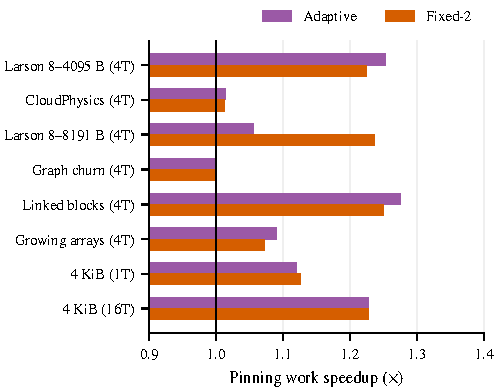
\includegraphics[width=\columnwidth]{pinning-work.pdf}
\caption{Pinning work speedup over matching unpinned indexed-plus-slab controls. Adaptive checks every 64 allocation-plus-free operations; fixed-2 retains at most two empty spans per class. T = tasklets; B = bytes; KiB = 1024 bytes.}
\label{fig:pinning-work}
\end{figure}

\begin{figure*}[!t]
\centering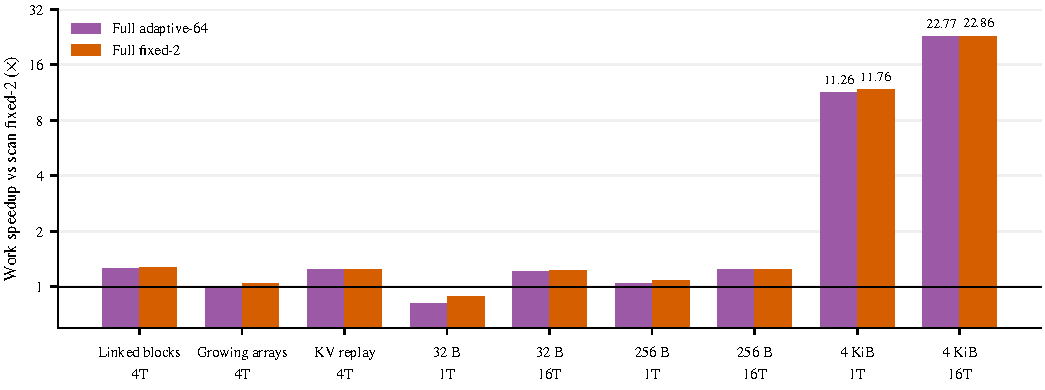
\includegraphics[width=\textwidth]{paper-workloads.pdf}
\caption{Full-stack policies on the nine paper-derived settings, with original request sizes. KV = key-value (allocation-only replay); T = tasklets; B = bytes; KiB = 1024 bytes. Adaptive-64 checks every 64 allocation-plus-free operations; fixed-2 retains at most two empty spans per class. Graphs are reduced ports.}
\label{fig:paper-workloads}
\end{figure*}

Graph churn gets 5.963-fold speedup from indexed fixed alone and 5.763-fold from the full fixed variant. Extra mechanisms do not improve its work phase further. Selection stays nearly unchanged. Full adaptive takes 19.172 ms on Larson 8--4095 B, compared with fixed's 16.255 ms. Adaptive bookkeeping and different refill/reclamation timing still matter after indexing and slabs are present.

Figure~\ref{fig:progression} shows why we keep every stage. Adding slabs to a workload with no eligible requests does not create a new gain. Similarly, the wider Larson range still has direct-bypass requests above 4 KiB. The complete design improves different paths, but its gains cannot be obtained by multiplying ratios from separate experiments.

\subsection{The effect of pinning metadata}
Figure~\ref{fig:pinning-work} compares each pinned variant with its matching unpinned slab variant. On Larson 8--4095 B, pinning adds 1.253-fold work speedup with adaptive retention and 1.224-fold with fixed retention. The corresponding CloudPhysics gains are 1.014 and 1.013. Wider Larson gains 1.056-fold with adaptive and 1.236-fold with fixed. Pinning barely changes churn work, but improves its total time by about 1.16--1.17-fold because initialization and final reclamation also call buddy.

The measured WRAM endpoint rises by 540 B. This comparison uses extra storage rather than equal WRAM budgets. Full-execution DRAM bytes fall by 46.48\% for fixed Larson 8--4095 B and 66.49\% for wider fixed Larson, but the work speedups are smaller. Some saved accesses occur outside work or outside its main bottleneck. A second Larson seed and another CloudPhysics window preserve similar incremental pinning gains.

On graph insertion and the original 4 KiB microbenchmark, pinning adds 1.250-fold work speedup on fixed linked blocks and 1.228-fold on fixed 4 KiB allocation at sixteen tasklets. On churn it saves 9.66\% of full-execution DRAM bytes with almost no work-time change. On the second Larson seed, its incremental gains are 1.219-fold adaptive and 1.231-fold fixed; on the second cache window they remain about 1.014-fold. This supports the metadata-placement mechanism while showing that traffic saved outside the main timed path has less effect on work time.

\subsection{Workloads from the paper}

Figure~\ref{fig:paper-workloads} shows the reduced graph ports, the original allocation-size settings and the KV allocation replay. Linked blocks improve from 19.330 to 15.198 ms with full fixed, or 1.272-fold. Growing arrays improve from 5.752 to 5.494 ms, or 1.047-fold, while full adaptive is slightly slower than baseline. These graphs contain no requests for the slab class. Their gains come from other parts of the allocator.

The 4 KiB allocation microbenchmark benefits most. Full fixed reduces one-tasklet work from 20.912 to 1.778 ms, or 11.763-fold. At sixteen tasklets it reduces 508.474 to 22.243 ms, or \textbf{22.860-fold}. Full adaptive reaches 22.766-fold. Backend allocations fall from 128 to 9 at one tasklet and from 2,048 to 144 at sixteen. Mean individual allocation latency at sixteen tasklets falls from 3960.865 to 166.665 microseconds with full fixed. The original frontend has no 4 KiB class, so these gains mainly show the value of serving a previously uncached size. They do not imply the same gain from enlarging existing small-object pages.

The one-tasklet 32 B case regresses from 0.875 to 0.990 ms with full fixed, or 0.884-fold speedup. Full adaptive takes 1.077 ms. In this small case the extra metadata work costs more than it saves. The KV allocation replay improves by about 1.24-fold, but this does not measure attention or serving performance.

\subsection{Total time and memory use}
Work speedup and total speedup answer different questions. In the one-tasklet 4 KiB case, full fixed improves work by 11.76-fold but total by 1.51-fold. Full-payload checking and the rest of the lifecycle occupy a large common share. At sixteen tasklets, total improves by 6.75-fold against 22.86-fold work. These are checked program totals in the simulator.

The same distinction appears in the other workloads. Larson 8--4095 B reaches 9.85-fold work and 6.77-fold total speedup. Graph churn reaches 5.76-fold work and 2.30-fold total. Wider Larson has 1.70-fold work and 1.86-fold total speedup because pinning also helps initialization and final free. Total can therefore improve more or less than work, depending on which phases benefit.

For configured Larson, full fixed reduces full-execution DRAM commands from 709,446 to 94,810. Its payload peak rises from 996 to 1,244 KiB. The sixteen-tasklet 4 KiB case reduces commands from 2,990,666 to 2,147,130, but payload reservation rises from 8 to 9 MiB. Indexed variants also need the separate 64 KiB ownership table. In the one-tasklet 32 B case, commands rise from 4,226 to 11,566. These costs explain why a larger allocator is not always faster or more memory-efficient.
\begin{table}[t]
\caption{Main-memory traffic and extra peak payload. B = scan fixed-2; PF = indexed + slabs + pinning with fixed-2. T = tasklets; MiB = $2^{20}$ bytes; KiB = $2^{10}$ bytes.}\label{tab:traffic}
\centering\small
\begin{tabular}{lrrr}\toprule
Case & B MiB & PF MiB & Peak +KiB \\ \midrule
Larson (4T) & 5.41 & 0.72 & +248 \\
Cache (4T) & 5.88 & 5.37 & +188 \\
Churn (4T) & 15.70 & 8.43 & 0 \\
4 KiB (16T) & 22.82 & 16.38 & +1024 \\
32 B (1T) & 0.032 & 0.088 & 0 \\
\bottomrule\end{tabular}
\par\vspace{2pt}{\footnotesize Peak is PF minus B; B in request sizes means bytes. The separate 64 KiB ownership map is excluded from payload peaks.}
\end{table}

Table~\ref{tab:traffic} summarizes representative memory costs. The complete fourteen-setting comparison is included in the accompanying result files. Counts include the whole execution, while timed allocations refer only to work. For example, the 4 KiB sixteen-tasklet benchmark issues 2,048 timed requests and needs only 144 slab backend allocations, yet it still transfers 16.38 MiB overall. Full-payload writes and checking remain after metadata calls have been reduced. Fewer backend calls therefore need not produce the same reduction in total bytes.

The final 98 configurations complete their offered work and fully coalesce the heap. The parent and paper-extension checks include 47 and 42 native test cases. Their maximum audited WRAM endpoints are 49,472 B and 48,296 B. The full numerical tables and memory counters accompany the submission.

\section{Discussion and Future Work}
The design addresses different costs at different points. Indexing reduces page discovery. The new class reduces repeated backend calls for medium-sized objects. Pinning speeds up metadata access in the backend calls that remain. Adaptive retention is useful when demand changes, while stable reuse often favors fixed retention.

The main limits are ownership and memory capacity. One tasklet cannot reclaim another inactive tasklet's pages. Large spans can waste space or fail under fragmentation. The graph sample is small and sparse, and the cache uses a selected trace window. All experiments use deterministic simulation. Testing a complete hardware image, broader traces and equal-WRAM metadata policies would make the results more useful. Separating check frequency from idle-decay duration would also make the adaptive policy easier to tune.

% Start the conclusion in the right column without forcing an extra page.
\makeatletter
\if@firstcolumn\newpage\fi
\makeatother

\section{Conclusion}
We extended PIM-malloc's software allocator with indexed allocation/free, fixed or adaptive empty retention, a 4 KiB slab class and pinned buddy metadata. The evaluation shows why these changes need separate controls. Each helps a particular part of allocation, while its metadata and memory costs remain visible on other workloads. Fixed retention is a strong choice for steady demand. Adaptation needs changing demand or memory pressure to justify its added work.

\noindent\textbf{Source code:} \url{https://github.com/mahaswint/cs5290}, directory \texttt{pim-reproduction/}.

\begin{thebibliography}{8}
\bibitem{pimmalloc} D. Lee, B. Hyun, Y. Kwon, and M. Rhu, ``PIM-malloc: A Fast and Scalable Dynamic Memory Allocator for Processing-In-Memory (PIM) Architectures,'' in \emph{HPCA}, 2026, doi: 10.1109/HPCA68181.2026.11408588.
\bibitem{artifact} VIA Research, ``PIM-malloc source code,'' commit \texttt{4fdcbcac3b0d}. [Online]. Available: \url{https://github.com/VIA-Research/PIM-malloc}
\bibitem{larson} P.-A. Larson and M. Krishnan, ``Memory Allocation for Long-Running Server Applications,'' in \emph{ISMM}, 1998, doi: 10.1145/286860.286880.
\bibitem{mimalloc} D. Leijen, B. Zorn, and L. de Moura, ``Mimalloc: Free List Sharding in Action,'' Microsoft Research, 2019. Benchmark code: \url{https://github.com/daanx/mimalloc-bench}
\bibitem{cloud} libCacheSim, ``CloudPhysics I/O sample,'' commit \texttt{c6ffd976c83d}. [Online]. Available: \url{https://github.com/1a1a11a/libCacheSim/blob/c6ffd976c83d9e731b37fc91e1ce930039f5ddb9/data/cloudPhysicsIO.csv}
\bibitem{faim} M. Winter et al., ``faimGraph: High Performance Management of Fully-Dynamic Graphs under Tight Memory Constraints on the GPU,'' in \emph{SC}, 2018. Code: \url{https://github.com/GPUPeople/faimGraph}
\bibitem{prim} CMU SAFARI, ``PrIM: Processing-in-Memory Benchmarks,'' commit \texttt{67179099730c}. [Online]. Available: \url{https://github.com/CMU-SAFARI/prim-benchmarks}
\end{thebibliography}
\end{document}
